% !TEX program = xelatex
% =========================================================================
% beamer-deck-template.tex — 学术会议 Beamer 模板（academic-ppt 技能内置资产）
% -------------------------------------------------------------------------
% 来源：IMHFC 2026 实战 deck（presentation_beamer.tex，多轮视觉验证通过），
%       泛化为「改内容即用」的骨架；每类帧型一份，占位内容本身即填写说明。
% 编译：latexmk -pdfxe beamer-deck-template.tex   （或 xelatex ×3）
%       默认「自建模式」零外部资产、直接可编译（白底，SKILL §2.2）。
% 用法：整份复制为 presentation.tex →
%       ① 改下方【色板】五处色值  ② 逐帧替换占位内容
%       ③ 有官方模板则按【背景三件套】注释切换  → 按 SKILL §4 视觉验证循环收尾。
% =========================================================================
\documentclass[aspectratio=169,11pt]{beamer}   % 16:9 = pptx 13.33″×7.5″，两边吻合无变形

\usepackage{fontspec}
\IfFontExistsTF{Helvetica Neue}{\setsansfont{Helvetica Neue}}{}   % 无则回退默认西文
\usefonttheme{professionalfonts}
\usepackage{amsmath}
\usepackage{unicode-math}
\IfFontExistsTF{Fira Math}{\setmathfont{Fira Math}}{}             % 无则回退默认数学字体
\usepackage{graphicx}
\usepackage{tikz}
\usetikzlibrary{positioning,arrows.meta}
\usepackage{booktabs}
\usepackage{array}
\usepackage{xcolor}
% \graphicspath{{figs/}}   % 论文原图统一放 figs/ 后取消注释

% =========================================================================
% 【色板】全场唯一需要改的五处——换色板即换风格（SKILL §2.2：单一主色 +
% 单一强调色 + 灰色辅助；反白字色块只做小面积强调，勿与白底正文大面积混排）
% =========================================================================
\definecolor{primary}{HTML}{0E2841}   % 主色（深蓝/navy 系）：标题、正文、结论块底
\definecolor{accent}{HTML}{E97132}    % 强调色（橙/teal 系）：编号、细线、关键词点缀
\definecolor{secondary}{HTML}{156082} % 辅助色：分组小标题、次级结构元素
\definecolor{muted}{HTML}{5A6B7B}     % 弱化灰：图例、脚注、副述
\definecolor{soft}{HTML}{F2F6F9}      % 浅底：卡片填充（实战验证五色，可直接沿用）

% ---- 干净版面 ----
\setbeamertemplate{navigation symbols}{}
\setbeamersize{text margin left=9mm, text margin right=9mm}
\setbeamercolor{normal text}{fg=primary}
\setbeamercolor{frametitle}{fg=primary}
\setbeamercolor{title}{fg=primary}
\setbeamercolor{structure}{fg=secondary}
\setbeamercolor{alerted text}{fg=accent}
\setbeamertemplate{itemize item}{\color{accent}\rule[0.45ex]{0.55ex}{0.55ex}}
\setbeamertemplate{itemize subitem}{\color{secondary}\rule[0.4ex]{0.4ex}{0.4ex}}
\setbeamertemplate{itemize subsubitem}{\color{secondary}\textendash}

% ---- 帧标题：主色粗体大标题 + 强调色细线；上方自动出现 SECTION 眉注 ----
% 眉注内容由 \divider 宏写入 \currentsection，无需手工维护
% ⚠️ 顶部 vspace 不可再压：眉注距页顶须留 ~4mm，投影 overscan 会裁掉贴边内容
\setbeamertemplate{frametitle}{%
  \nointerlineskip\vspace{4mm}%
  \begin{beamercolorbox}[wd=\paperwidth,leftskip=9mm,rightskip=9mm]{frametitle}%
    {\ifx\currentsection\empty\else\color{accent}\scriptsize\bfseries\currentsection\par\vspace{0.3mm}\fi}%
    \usebeamerfont{frametitle}\bfseries\insertframetitle\\[-2mm]%
    {\color{accent}\rule{13mm}{1.1pt}}%
  \end{beamercolorbox}%
}
\setbeamerfont{frametitle}{size=\Large,series=\bfseries}

% =========================================================================
% 【背景三件套】官方模板模式：解压会议 pptx 取 ppt/media/ 三张背景图放入
% figs/beamer_bg/，把三个宏改为 \includegraphics[width=\paperwidth,
% height=\paperheight,keepaspectratio=false]{beamer_bg/bg_xxx}（SKILL §2.1）。
% 自建模式（默认）：三个宏留空 = 白底，天然避开 \usebackgroundtemplate
% 优先级坑与 pptx→Beamer 单位换算坑（SKILL §2.1/§2.2）。
% ⚠️ 若官方背景底部有品牌条带：按百分比换算条带高度（Beamer 169 纸高仅 9cm，
% 底部 9.76% 条带 ≈ 8.8mm），并按下一段 footline 注释预留，勿删背景（SKILL §7）。
% =========================================================================
\newcommand{\BgCover}{}
\newcommand{\BgContent}{}
\newcommand{\BgClosing}{}
\usebackgroundtemplate{\BgContent}

% ---- footline：运行标题 + 页码 ----
% 官方模板有底部条带时的避让参数（实战验证）：ht+dp = 11mm 预留，正文止于
% 条带上方 ~2mm，页码基线落在条带内；自建白底模式同样可用，无需改动
\setbeamertemplate{footline}{%
  \begin{beamercolorbox}[wd=\paperwidth,ht=7mm,dp=4mm,leftskip=9mm,rightskip=9mm]{}%
    \hbox to\dimexpr\paperwidth-18mm\relax{%
      \hfill
      {\color{primary}\scriptsize\bfseries Running title --- replace or delete}% 运行标题，可留空
      \hfill
      \llap{{\color{primary}\scriptsize\insertframenumber\,/\,\inserttotalframenumber}}}%
  \end{beamercolorbox}}

% =========================================================================
% 可复用宏（实战验证，勿改几何参数）
% =========================================================================
% ---- 转场页：#1 大编号("01")  #2 节序号("1")  #3 标题  #4 一句话副述 ----
% 同时把 SECTION 眉注写入 \currentsection，后续内容页自动带眉注
\newcommand{\divider}[4]{%
  \renewcommand{\currentsection}{SECTION #2: #3}%
  \begin{frame}[plain]
    \begin{tikzpicture}[remember picture, overlay]
      % 大编号（强调色，居中偏上）
      \node[text=accent, font=\bfseries\fontsize{40}{40}\selectfont, inner sep=0]
        at ([yshift=14mm]current page.center) {#1};
      % 短横线
      \draw[accent, line width=1.2pt]
        ([xshift=-20mm,yshift=7mm]current page.center) -- ([xshift=20mm,yshift=7mm]current page.center);
      % 标题（主色粗体居中）
      \node[text width=130mm, align=center, inner sep=0]
        at ([yshift=-3mm]current page.center){%
        {\color{primary}\bfseries\LARGE #3}};
      % 副述（辅助色斜体）
      \node[text width=130mm, align=center, inner sep=0]
        at ([yshift=-16mm]current page.center){%
        {\color{secondary}\itshape\small #4}};
    \end{tikzpicture}
  \end{frame}%
}

% ---- 强调卡片：\callout[底色]{文本宽}{内容}（默认底色 primary）----
% ⚠️ 宽度规则：文本宽 + 2×3mm 内边距 必须小于所在列宽（SKILL §3）
\newcommand{\callout}[3][primary]{%
  \begin{tikzpicture}\node[fill=#1, rounded corners=2pt, inner sep=3mm, text width=#2, align=left]{#3};\end{tikzpicture}}

\title{}\author{}\date{}   % 封面手工排版，不用 \titlepage
\newcommand{\currentsection}{}   % SECTION 眉注载体，由 \divider 维护
\newcommand{\BgNone}{}   % 封底模式判断哨兵：\ifx\BgClosing\BgNone 仅在 \BgClosing 为空时成立
                         % （\newcommand 定义的宏是 \long，与 \empty 的 \ifx 比较永不相等，勿改用 \empty）

\begin{document}

% =========================================================================
% 帧型 1：封面（bg_cover / 自建模式下白底）
% 布局：标题区锚在页面左上偏右（xshift=52mm 给左侧留出照片/校徽区）
% =========================================================================
{\usebackgroundtemplate{\BgCover}%
\begin{frame}[plain]
\begin{tikzpicture}[remember picture, overlay]
  \node[anchor=north west, text width=100mm, align=left, inner sep=0]
    at ([xshift=52mm,yshift=-20mm]current page.north west){%
    {\color{primary}\bfseries\LARGE Paper title over at most two lines}\\[2.5mm]
    {\color{secondary}\itshape\normalsize Subtitle: method or angle in one line}\\[5mm]
    {\color{primary}\small Author One \,\textbullet\, Author Two \,\textbullet\, Author Three$^*$}\\[2.5mm]
    {\color{muted}\footnotesize Affiliation One \,\textbullet\, Affiliation Two}\\[3.5mm]
    {\color{accent}\bfseries\footnotesize CONF 2026 \,\textbullet\, Month Day--Day, 2026 \,\textbullet\, City, Country}};
\end{tikzpicture}
\end{frame}}

% =========================================================================
% 帧型 2：目录（每节一条浅底卡片 = 大编号 + 粗标题 + 灰色一句话副述）
% =========================================================================
\begin{frame}{Outline}
\callout[soft]{136mm}{{\color{accent}\bfseries\Large 01}\hspace{4mm}{\color{primary}\bfseries\large Introduction}\hspace{4mm}{\color{muted}\footnotesize One-line description of part one.}}

\vspace{2.5mm}
\callout[soft]{136mm}{{\color{accent}\bfseries\Large 02}\hspace{4mm}{\color{primary}\bfseries\large Model}\hspace{4mm}{\color{muted}\footnotesize One-line description of part two.}}

\vspace{2.5mm}
\callout[soft]{136mm}{{\color{accent}\bfseries\Large 03}\hspace{4mm}{\color{primary}\bfseries\large System}\hspace{4mm}{\color{muted}\footnotesize One-line description of part three.}}

\vspace{2.5mm}
\callout[soft]{136mm}{{\color{accent}\bfseries\Large 04}\hspace{4mm}{\color{primary}\bfseries\large Results}\hspace{4mm}{\color{muted}\footnotesize One-line description of part four.}}
\end{frame}

% ---- 每个章节开始处插一页转场；眉注随 #2/#3 自动更新 ----
\divider{01}{1}{Introduction}{One sentence on why this problem matters and where the bottleneck lies.}

% =========================================================================
% 帧型 3：纯文字要点页（itemize + 底部 key-insight 结论块）
% 注意：纯文字页不配色块卡片，橙色小标题 + \alert 点缀即可（SKILL §3）
% =========================================================================
\begin{frame}{Plain bullets frame: state the frame title as a claim}
\footnotesize
\begin{itemize}\setlength\itemsep{1.5mm}
\item One point = one message: state the fact first, then its consequence.
\item Quantify where possible; numbers beat adjectives in review rooms.
\item Use \alert{accent} only on the two or three words that carry the argument.
\item Close the frame with the takeaway, not with a detail.
\end{itemize}
\vspace{3mm}
\callout{136mm}{\color{accent}\footnotesize\bfseries Key insight:\ \ \color{white}one sentence the audience must remember from this frame --- stated, not hinted.}
\end{frame}

% =========================================================================
% 帧型 4：三卡片页（研究缺口/贡献/角色分工等并列语义）
% 实战安全组合：39mm 卡片文本宽 配 0.32\textwidth 列（42mm 会溢出 7pt）
% =========================================================================
\begin{frame}{Three-card frame: three parallel streams or contributions}
\footnotesize
\begin{columns}[T]
\begin{column}{0.32\textwidth}
\callout[soft]{39mm}{\color{secondary}\bfseries 1\quad First card\\[1.5mm]\color{primary} Two to four lines describing stream one.}
\end{column}
\begin{column}{0.32\textwidth}
\callout[soft]{39mm}{\color{secondary}\bfseries 2\quad Second card\\[1.5mm]\color{primary} Two to four lines describing stream two.}
\end{column}
\begin{column}{0.32\textwidth}
\callout[soft]{39mm}{\color{secondary}\bfseries 3\quad Third card\\[1.5mm]\color{primary} Two to four lines describing stream three.}
\end{column}
\end{columns}
\vspace{3.5mm}
\callout{136mm}{\color{accent}\footnotesize\bfseries Shared limitation:\ \ \color{white}the one sentence that motivates your work, following the three cards.}
\end{frame}

% =========================================================================
% 帧型 5：通栏纵排页（多列长文字的替代：每行 = 大编号 + 粗标题 + 灰色小注）
% =========================================================================
\begin{frame}{Vertical list frame: long texts read better in full-width rows}
\small
\callout[soft]{136mm}{{\color{accent}\bfseries\Large 1}\hspace{4mm}{\color{primary}\bfseries First item headline}\hspace{4mm}{\color{muted}\footnotesize Grey sub-note in one line.}}
\vspace{2.5mm}
\callout[soft]{136mm}{{\color{accent}\bfseries\Large 2}\hspace{4mm}{\color{primary}\bfseries Second item headline}\hspace{4mm}{\color{muted}\footnotesize Grey sub-note in one line.}}
\vspace{2.5mm}
\callout[soft]{136mm}{{\color{accent}\bfseries\Large 3}\hspace{4mm}{\color{primary}\bfseries Third item headline}\hspace{4mm}{\color{muted}\footnotesize Grey sub-note in one line.}}
\end{frame}

% =========================================================================
% 帧型 6：左文右图页（阅读顺序自然，SKILL §3）
% ⚠️ includegraphics 带 width+height 双约束 + keepaspectratio：放大图时若被
% 列宽卡住，调 height 无效，要改列宽（实战 0.46→0.54 放大 37%，SKILL §3）
% =========================================================================
\begin{frame}{Figure frame: text left, figure right}
\footnotesize
\begin{columns}[T]
\begin{column}{0.50\textwidth}
\centering
% 换成论文原图（矢量 PDF 优先）：
% \includegraphics[width=\linewidth,height=0.6\textheight,keepaspectratio]{fig1}
\fbox{\parbox[c][0.55\textheight][c]{0.88\linewidth}{\centering\color{muted}Paper figure placeholder\\ replace with \texttt{\textbackslash includegraphics}}}
\end{column}
\begin{column}{0.48\textwidth}
\textcolor{secondary}{\bfseries Group head}\quad short setup sentence.
\begin{itemize}\setlength\itemsep{0.3mm}
\item Dense annotations go here in scriptsize.
\item \alert{Highlight} the one arc/rule that matters most.
\end{itemize}
\textcolor{secondary}{\bfseries Second group head}\quad more structure.
\callout[accent]{52mm}{\color{white}\scriptsize\bfseries Goal: one-line objective or takeaway card}
\end{column}
\end{columns}
\end{frame}

% =========================================================================
% 帧型 7：左文右示意图页（小型 TikZ 原理图 + 底部双色图例）
% =========================================================================
\begin{frame}{Diagram frame: text left, schematic right}
\footnotesize
\begin{columns}[T]
\begin{column}{0.54\textwidth}
Explain the mechanism in prose; bold the arc names in \textcolor{accent}{\bfseries accent}:
\begin{itemize}\setlength\itemsep{1mm}
\item \textcolor{accent}{\bfseries Flow one} $(i,t)\to(j,t{+}\tau)$ --- what it carries.
\item \textcolor{accent}{\bfseries Flow two} --- what it carries.
\item \textcolor{accent}{\bfseries Flow three} --- what it carries.
\end{itemize}
$\Rightarrow$ the one-line conclusion of the mechanism.
\end{column}
\begin{column}{0.42\textwidth}
\centering
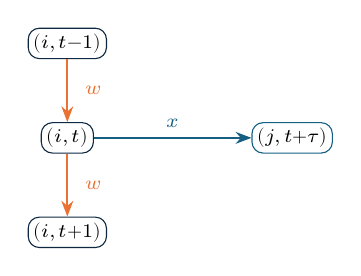
\begin{tikzpicture}[every node/.style={font=\scriptsize}, >={Stealth[length=2mm]}]
 \node[draw=primary,rounded corners,inner sep=2pt] (a) {$(i,t{-}1)$};
 \node[draw=primary,rounded corners,inner sep=2pt,below=8mm of a] (b) {$(i,t)$};
 \node[draw=primary,rounded corners,inner sep=2pt,below=8mm of b] (c) {$(i,t{+}1)$};
 \node[draw=secondary,rounded corners,inner sep=2pt,right=20mm of b] (d) {$(j,t{+}\tau)$};
 \draw[->,accent,thick] (a) -- node[right=1mm]{$w$} (b);
 \draw[->,accent,thick] (b) -- node[right=1mm]{$w$} (c);
 \draw[->,secondary,thick] (b) -- node[above]{$x$} (d);
\end{tikzpicture}\\[2mm]
{\color{muted}\scriptsize \textcolor{accent}{\rule{2mm}{1.2mm}}~flow two\ \ \textcolor{secondary}{\rule{2mm}{1.2mm}}~flow one}
\end{column}
\end{columns}
\end{frame}

% =========================================================================
% 帧型 8：表格+列表双栏页（左表右释；booktabs 三线表，字号 footnotesize）
% =========================================================================
\begin{frame}{Table frame: table left, reading right}
\small
\begin{columns}[T]
\begin{column}{0.46\textwidth}
\textcolor{secondary}{\bfseries Table head}\\[1mm]
\centering
\setlength{\tabcolsep}{6pt}\renewcommand{\arraystretch}{1.2}
\begin{tabular}{@{}lccc@{}}
\toprule
Type & a & b & c \\
\midrule
Row one   & 1 & 2 & \alert{0.25} \\
Row two   & 2 & 4 & \alert{0.5} \\
Row three & 3 & 6 & 1 \\
\bottomrule
\end{tabular}\\[1.5mm]
\footnotesize One-line caption; note the \alert{highlighted} entries.
\end{column}
\begin{column}{0.50\textwidth}
\textcolor{secondary}{\bfseries Assumptions / reading}
\begin{enumerate}\setlength\itemsep{1.2mm}\footnotesize
\item First assumption, stated so a reviewer can attack it.
\item Second assumption; name what it buys you.
\item Third assumption and its boundary.
\end{enumerate}
\end{column}
\end{columns}
\end{frame}

% =========================================================================
% 帧型 9：数学页 1/2（目标函数+约束组；底部灰色符号图例行必备，SKILL §3）
% ⚠️ 数学页必须与论文逐项核对：系数、求和域、整型标记（SKILL §3 实战抓漏）
% =========================================================================
\begin{frame}{Mathematical model (1/2): objective \& conservation}
\footnotesize
\textcolor{secondary}{\bfseries Objective} --- charge each flow with its unit cost and footprint:
\begin{align*}
\min\ \ & \sum_{t,(i,j)\in\mathcal A}\sum_g c^{\mathrm{f}}_{ij}\theta_g\,x^{t}_{ijg}
+\sum_{t,i,g} c^{\mathrm{h}}_i\theta_g\,w^{t}_{ig}
+\sum_{t,i,g} c^{\mathrm{r}}_i\theta_g\,r^{t}_{ig}
\end{align*}
\textcolor{secondary}{\bfseries Flow conservation} at every vertex, one line per node class:
\begin{align*}
w^{t-1}_{ig}{+}S^{t}_{ig}{+}r^{t}_{ig} &=\, y^{t}_{ig}{+}w^{t}_{ig}{+}{\scriptstyle\sum_{\mathcal A_i^+}}x^{t} && \text{depots } i\in D\\
S^{t}_{pg} &=\, {\textstyle\sum_{\mathcal A_p^+}}x^{t} && \text{sources } p\in P\\
{\textstyle\sum_{\mathcal A_q^-}}x^{t} &=\, y^{t}_{qg} && \text{sinks } q\in Q
\end{align*}
{\color{muted}\scriptsize Notation:\ $x$ flow $\cdot$ $w$ inventory $\cdot$ $r$ rent $\cdot$ $S$ supply $\cdot$ $y$ service $\cdot$ $\theta_g$ footprint $\cdot$ $\mathcal A^{\pm}_i$ out-/in-arcs of $i$}
\end{frame}

% =========================================================================
% 帧型 10：数学页 2/2（耦合与边界条件：橙色 [LABEL] 眉标分块 + 整型注脚）
% =========================================================================
\begin{frame}{Mathematical model (2/2): couplings \& boundary conditions}
\footnotesize
{\color{accent}\scriptsize\bfseries [COUPLING A]}\ \ \textcolor{secondary}{\bfseries What binds the types together} --- one sentence on its role:
\[
\sum_{g} x^{t}_{ijg} \;=\; D^{t}_{i}\qquad \forall\,i,\ t
\]
{\color{accent}\scriptsize\bfseries [COUPLING B]}\ \ \textcolor{secondary}{\bfseries Shared capacity} --- one budget across all types:
\[
\sum_{g}\theta_g\, x^{t}_{ijg}\le F^{\max}_{ij}\ \ (\text{arc})\qquad\qquad \sum_{g}\theta_g\, w^{t}_{ig}\le U^{\max}_{i}\ \ (\text{node})
\]
{\color{accent}\scriptsize\bfseries [BOUNDARY]}\ \ \textcolor{secondary}{\bfseries Terminal condition} --- rule out end-of-horizon artifacts:
\[
w^{T}_{ig}\ge \bar I_{ig}\qquad(\text{set } \bar I_{ig}=I^{0}_{ig}\ \Rightarrow\ \text{no-net-depletion})
\]
{\color{muted}\scriptsize Integrality: $x^{t}_{ijg},\,w^{t}_{ig},\,r^{t}_{ig},\,y^{t}_{ig}\in\mathbb Z_+$ --- units are discrete; initial state $w^{0}_{ig}{=}I^{0}_{ig}$ fixed.}
\vspace{0.5mm}
\callout[secondary]{136mm}{\color{white}\footnotesize\bfseries One sentence on why this model is genuinely the coupled one --- remove the named couplings and it splits apart.}
\end{frame}

% =========================================================================
% 帧型 11：系统总览页（TikZ overlay 绝对定位：左上文字面板 + 右下大图）
% ⚠️ 图占位行换成 \includegraphics[height=66mm,keepaspectratio]{architecture}
% =========================================================================
\begin{frame}{Overview frame: pinned panel + figure}
\begin{tikzpicture}[remember picture, overlay]
  % 文字面板——钉在帧标题下方左侧（宽 57mm，右侧给图留 ≥6mm 空隙）
  \node[anchor=north west, text width=57mm, inner sep=0]
    at ([xshift=9mm,yshift=-24mm]current page.north west)
    {{\color{accent}\bfseries Panel headline}\\[1.5mm]
    {\footnotesize Two to five lines positioning the figure: what is grounded by what, and what makes it robust.\\[1.5mm]
    \itshape The italic kicker line that states the design philosophy.}};
  % 大图——钉在右下（46mm 高为安全上限：再高会压帧标题；换图时只动 height）
  \node[anchor=south east, inner sep=0]
    at ([xshift=-10mm,yshift=14mm]current page.south east)
    {\fbox{\parbox[c][46mm][c]{74mm}{\centering\color{muted}Overview figure placeholder\\ architecture figure}}};
\end{tikzpicture}
\end{frame}

% =========================================================================
% 帧型 12：表格+结论横幅页（症状→归因→动作类内容）
% =========================================================================
\begin{frame}{Routing-table frame: symptom, stage, action}
\small
One framing sentence above the table:
\vspace{2mm}

\centering
\setlength{\tabcolsep}{5pt}\renewcommand{\arraystretch}{1.25}
\begin{tabular}{@{}p{44mm} p{40mm} p{49mm}@{}}
\toprule
\textcolor{secondary}{\bfseries Symptom} & \textcolor{secondary}{\bfseries Where} & \textcolor{secondary}{\bfseries Action} \\
\midrule
symptom one & stage one & action one \\
symptom two & stage two & action two \\
symptom three & stage three & action three \\
\bottomrule
\end{tabular}
\vspace{3mm}

\callout{136mm}{\color{accent}\footnotesize\bfseries Complementary by design:\ \ \color{white}one closing sentence that pairs the two mechanisms on this frame.}
\end{frame}

% =========================================================================
% 帧型 13：结果大数字页（左：主色大数字卡；右：等价性/稳健性要点）
% =========================================================================
\begin{frame}{Result 1 --- headline number with evidence}
\begin{columns}[T]
\begin{column}{0.46\textwidth}
\centering

\begin{tikzpicture}
\node[fill=primary, rounded corners=2pt, inner sep=3mm, text width=58mm, align=center]{%
\color{white}\Huge\bfseries 1{,}234{,}567.8\\[1.5mm]
\color{accent}\large\bfseries the claim in three words\\[1mm]
\color{soft}\footnotesize qualifier (gap $<10^{-6}$, MIPGap$=0$)};
\end{tikzpicture}
\end{column}
\begin{column}{0.52\textwidth}
\footnotesize
\textcolor{secondary}{\bfseries Why the number is trustworthy:}
\begin{itemize}\setlength\itemsep{0.6mm}
\item Identical size: $1317\times 2740$, 7556 nonzeros
\item Identical structure after presolve
\item Differences only in iteration counts --- a code-level artifact
\item Same final plan / decision vector
\end{itemize}
\vspace{1mm}
{\color{accent}\bfseries $\Rightarrow$\ One-sentence takeaway.}
\end{column}
\end{columns}
\end{frame}

% =========================================================================
% 帧型 14：图+结果表+大数字卡页（左图右表，右下主色数字卡）
% =========================================================================
\begin{frame}{Result 2 --- scenario comparison}
\begin{columns}[T]
\begin{column}{0.50\textwidth}
\centering
% \includegraphics[width=\linewidth]{fig5}\\[1mm]
\fbox{\parbox[c][40mm][c]{0.9\linewidth}{\centering\color{muted}Scenario bar-chart placeholder}}\\[1mm]
{\color{muted}\scriptsize Axis label and unit, one line}
\end{column}
\begin{column}{0.48\textwidth}
\footnotesize
\setlength{\tabcolsep}{4pt}\renewcommand{\arraystretch}{1.25}
\begin{tabular}{@{}p{34mm}r c@{}}
\toprule
\textbf{Scenario} & \textbf{Total} & \textbf{$\Delta$} \\
\midrule
S1\ Baseline     & 1{,}234{,}567 & --- \\
S2\ No channel A & 1{,}320{,}000 & {\color{accent}\bfseries +7.0\,\%} \\
S3\ No channel B & 1{,}490{,}000 & {\color{accent}\bfseries +20.7\,\%} \\
\bottomrule
\end{tabular}\\[2.5mm]

\begin{tikzpicture}
\node[fill=primary, rounded corners=2pt, inner sep=3mm, text width=61mm, align=left]{%
\color{accent}\Large\bfseries +27.9\,\%\ \ {\color{white}\footnotesize total cost if both channels are disabled}\\[1.5mm]
\color{soft}\scriptsize Which channel dominates, in one line.};
\end{tikzpicture}
\end{column}
\end{columns}
\end{frame}

% =========================================================================
% 帧型 15：成本构成/管理启示双栏页
% =========================================================================
\begin{frame}{Composition \& insights}
\small
\begin{columns}[T]
\begin{column}{0.48\textwidth}
\textcolor{secondary}{\bfseries Where the budget goes}
\begin{itemize}\setlength\itemsep{0.8mm}\footnotesize
\item Component one \alert{62\,\%} --- driven by what
\item Component two \alert{19.5\,\%} --- residual role
\item Component three \alert{18\,\%}
\item Component four \alert{$<1\,\%$}
\end{itemize}
\textcolor{secondary}{\bfseries What varies across scenarios}\\
\footnotesize Only the dominant component responds --- so the lever's value lands where the cost is.
\end{column}
\begin{column}{0.48\textwidth}
\textcolor{accent}{\bfseries Where to prioritize}\\[1.5mm]
\footnotesize Name the dominant lever and its share (\textbf{50\,\%}).\\[1.5mm]
Give the per-unit saving numbers.\\[1.5mm]
\itshape $\Rightarrow$ Managerial message: with modeling automated, planner attention is best spent framing the scenario, not hand-crafting the model.
\end{column}
\end{columns}
\end{frame}

% =========================================================================
% 帧型 16：结论双栏页（左：做了什么；右：贡献定位 + future work）
% =========================================================================
\begin{frame}{Conclusion \& future work}
\begin{columns}[T]
\begin{column}{0.48\textwidth}
\small
\textcolor{accent}{\bfseries What we did}
\begin{itemize}\setlength\itemsep{0.9mm}
\item The system in one line: input $\to$ output.
\item Its three parts, in three short bullets.
\item Validation result on the real case.
\item The operational finding, with its number.
\end{itemize}
\end{column}
\begin{column}{0.48\textwidth}
\small
\textcolor{secondary}{\bfseries Positioning}\\[1mm]
\footnotesize Where this sits in the field, in two lines.\\[2.5mm]
\textcolor{accent}{\bfseries Future work}\\[1mm]
\footnotesize Direction one; direction two; direction three.
\end{column}
\end{columns}
\end{frame}

% =========================================================================
% 帧型 17：封底（bg_closing / 自建模式白底）
% ⚠️ 官方封底背景通常自带致谢字样（实测某会议 bg_closing 已印 "Thank you for your
% attention!"，占页高 ~30-46%），整块叠字必乱码——实战原版就曾叠印。故封底
% 模式自适应：白底显示完整致谢块；官方背景只留单行联系信息，落在实测空档
% （实测例为页高 46-54%，此处 yshift=-1mm ≈ 页高中心）；换会议背景时按其
% 留白重调 yshift，勿信默认居中
% =========================================================================
{\usebackgroundtemplate{\BgClosing}%
\begin{frame}[plain]
\begin{tikzpicture}[remember picture, overlay]
  \ifx\BgClosing\BgNone
    % 自建白底（\BgClosing 为空）：完整致谢块居中
    \node[anchor=center, text width=120mm, align=center] at (current page.center){%
      {\color{primary}\bfseries\Huge Thank you!}\\[4mm]%
      {\color{primary}\large Questions \& discussion}\\[6mm]%
      {\color{accent}\bfseries\normalsize Presenter \,\textbullet\, email@institution.edu}\\[1.5mm]%
      {\color{muted}\footnotesize Institution}};
  \else
    % 官方背景：背景已含致谢字样，只留单行联系方式
    \node[anchor=center, text width=140mm, align=center] at ([yshift=-1mm]current page.center){%
      {\color{accent}\bfseries\footnotesize Presenter \,\textbullet\, email@institution.edu \,\textbullet\, Institution}};
  \fi
\end{tikzpicture}
\end{frame}}

\end{document}
